\section{Footstep Evaluation Network}

The results of the Footstep Evaluation Network are highly promising,
with the model able to predict footstep candidate maps with strong
accuracy. \autoref{fig:data-cn-typical-comparison} shows the model
output alongside the ground truth for a typical data sample.

\autoref{fig:data-cn-challenging-comparison} illustrates a
particularly challenging sample, in which the model still
successfully identifies the most suitable positions for each leg.
Notably, the back-left leg must be positioned far from its nominal
location to maintain stability in this scenario, and the model
correctly predicts this adjustment.

In the context of this work, the precise accuracy of the model is not
critical. Its primary role is to sample the continuous space of foot
positions to generate candidate actions for the GaitNet policy.

\begin{figure}[H]
  \centering
  \begin{minipage}[T]{0.45\textwidth}
    \centering
    \includegraphics[width=\textwidth]{images/data/training/typical-expected.png}
  \end{minipage}
  \hfill
  \begin{minipage}[T]{0.45\textwidth}
    \centering
    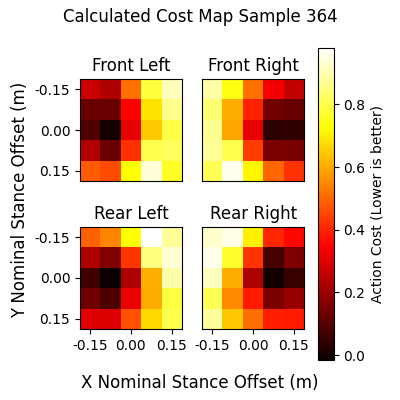
\includegraphics[width=\textwidth]{images/data/training/typical-calculated.png}
  \end{minipage}
  \hfill

  \caption{Typical data samples showing calculated (left) and
  expected (right) quadruped images.}
  \label{fig:data-cn-typical-comparison}
\end{figure}

\begin{figure}[H]
  \centering
  \begin{minipage}[T]{0.45\textwidth}
    \centering
    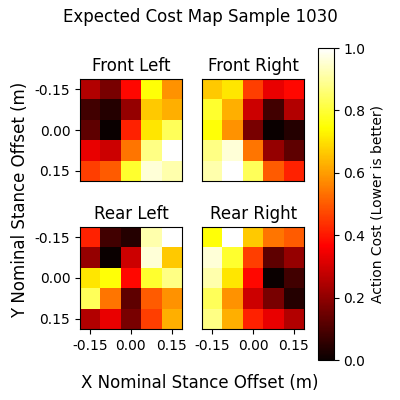
\includegraphics[width=\textwidth]{images/data/training/challenging-expected.png}
  \end{minipage}
  \hfill
  \begin{minipage}[T]{0.45\textwidth}
    \centering
    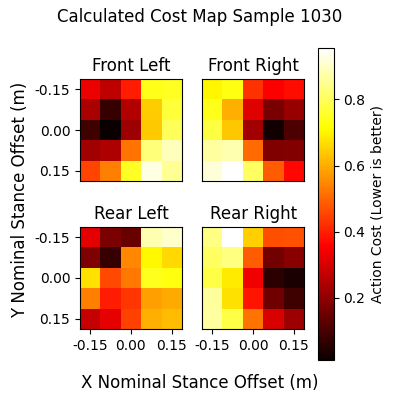
\includegraphics[width=\textwidth]{images/data/training/challenging-calculated.png}
  \end{minipage}
  \hfill

  \caption{Particularly challenging data samples showing calculated (left) and
  expected (right) quadruped images.}
  \label{fig:data-cn-challenging-comparison}
\end{figure}

\begin{todo}
  Provide results showing how the model performs in situations like
  those   in \cite{bratta_contactnet_2024} (single foot steps on our
  terrain).   This should highlight that this is a correct
  implementation of their method.
\end{todo}
